\imprimircapa
\imprimirfolhaderosto*

\begin{fichacatalografica}
    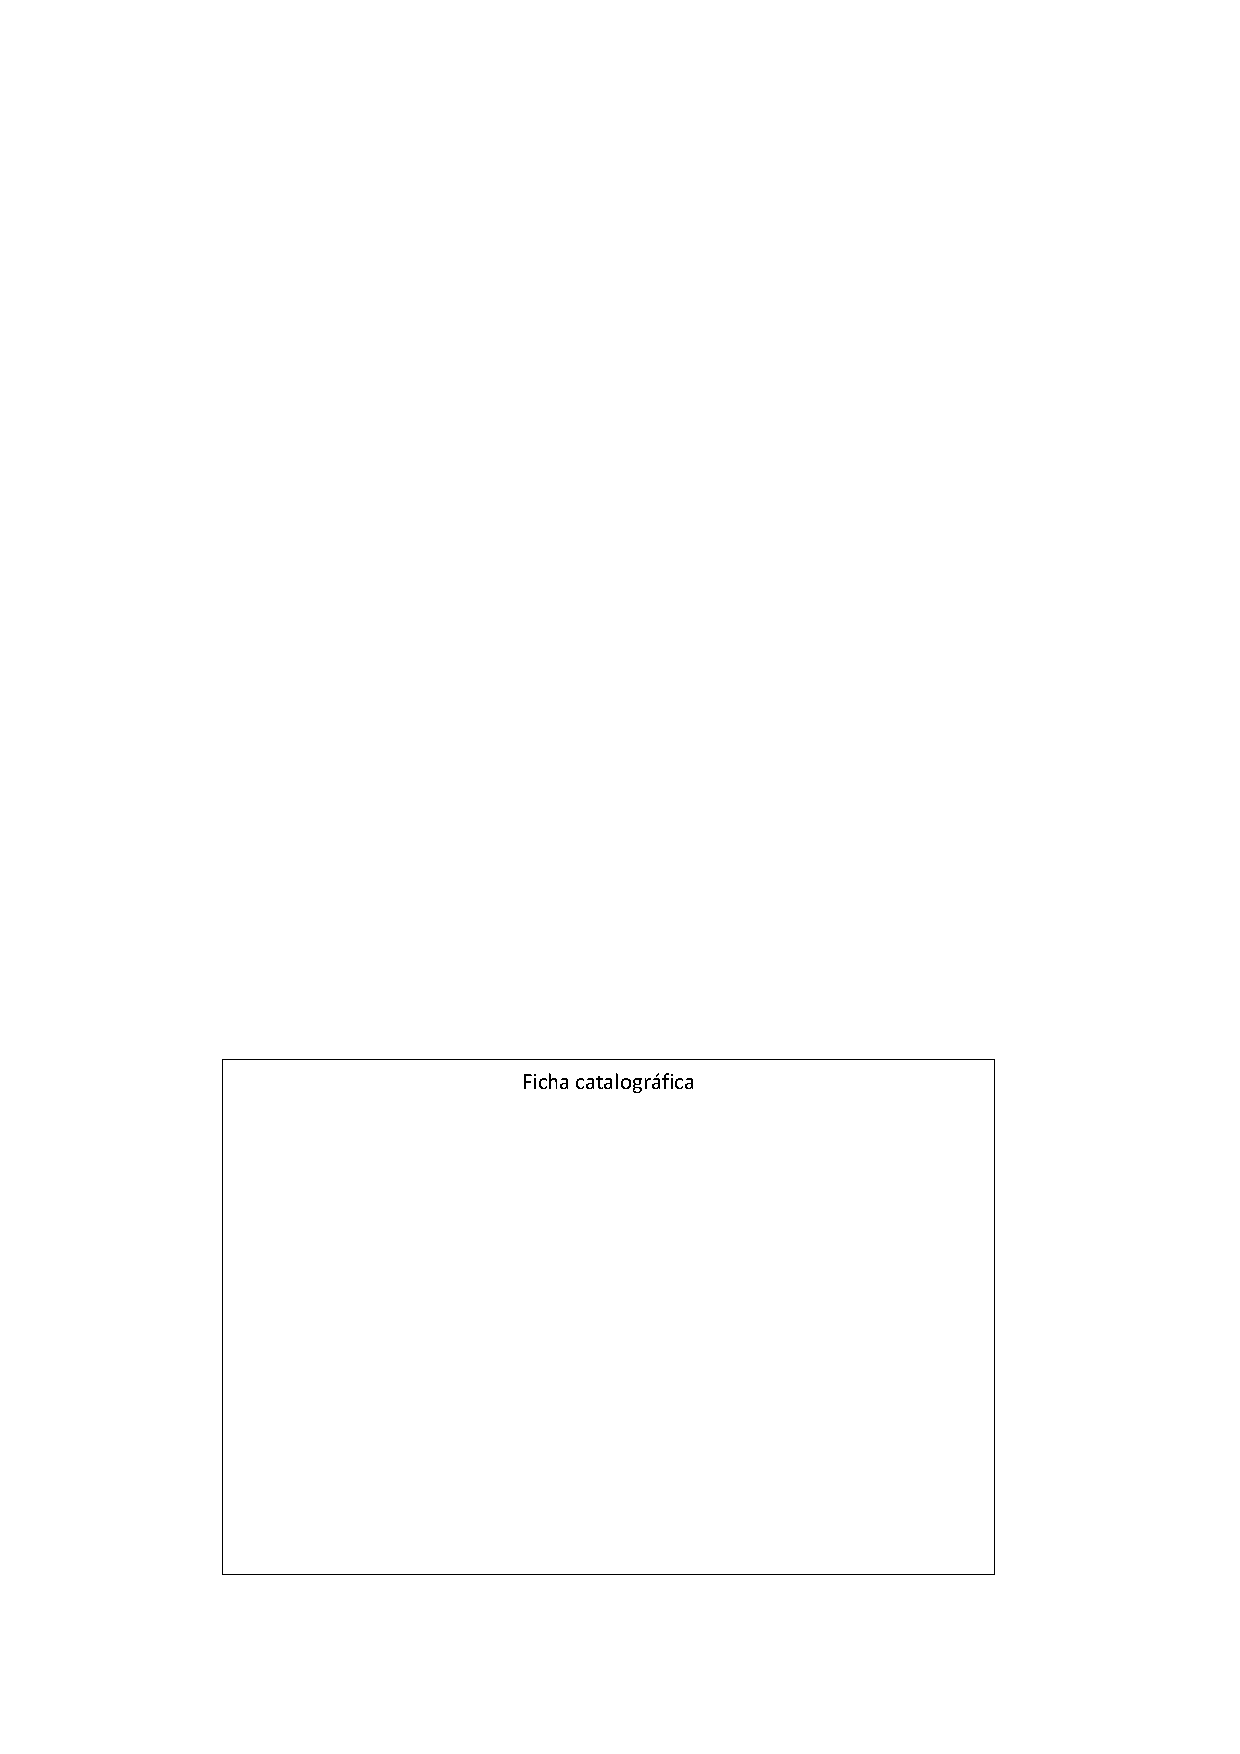
\includepdf{ficha_catalografica.pdf}
\end{fichacatalografica}

\begin{folhadeaprovacao}

	\noindent Dissertação de autoria de Henrique Abrantes Vitoi, sob o título \textbf{``\imprimirtitulo''}, apresentada à Escola Politécnica da Universidade de São Paulo, para obtenção do título de Mestre em Ciências pelo Programa de Pós-graduação em Engenharia Mecânica, na área de concentração Engenharia de Controle e Automação Mecânica, aprovada em \_\_\_\_\_\_\_ de \_\_\_\_\_\_\_\_\_\_\_\_\_\_\_\_\_\_\_\_\_\_ de \_\_\_\_\_\_\_\_\_\_ pela comissão julgadora constituída pelos doutores:
	\vspace*{3cm}
	\begin{center}
		\_\_\_\_\_\_\_\_\_\_\_\_\_\_\_\_\_\_\_\_\_\_\_\_\_\_\_\_\_\_\_\_\_\_\_\_\_\_\_\_\_\_\_\_\_\_\_\_\_\_\_\_\_\_\_\_
		\vspace*{0.2cm} 
		\\ \textbf{Prof. Dr. \_\_\_\_\_\_\_\_\_\_\_\_\_\_\_\_\_\_\_\_\_\_\_\_\_\_\_\_\_\_\_\_\_\_\_\_\_\_\_\_\_\_\_\_\_\_\_\_\_\_\_\_\_\_\_\_\_\_\_\_\_\_} 
		\\ \vspace*{0.2cm} 
		Instituição: \_\_\_\_\_\_\_\_\_\_\_\_\_\_\_\_\_\_\_\_\_\_\_\_\_\_\_\_\_\_\_\_\_\_\_\_\_\_\_\_\_\_\_\_\_\_\_\_\_\_\_\_\_\_\_\_\_\_ 
		\\ \vspace*{0.2cm}
		Presidente 

		\vspace*{2cm}

		\_\_\_\_\_\_\_\_\_\_\_\_\_\_\_\_\_\_\_\_\_\_\_\_\_\_\_\_\_\_\_\_\_\_\_\_\_\_\_\_\_\_\_\_\_\_\_\_\_\_\_\_\_\_\_\_
		\vspace*{0.2cm} 
		\\ \textbf{Prof. Dr. \_\_\_\_\_\_\_\_\_\_\_\_\_\_\_\_\_\_\_\_\_\_\_\_\_\_\_\_\_\_\_\_\_\_\_\_\_\_\_\_\_\_\_\_\_\_\_\_\_\_\_\_\_\_\_\_\_\_\_\_\_\_} 
		\\ \vspace*{0.2cm} 
		Instituição: \_\_\_\_\_\_\_\_\_\_\_\_\_\_\_\_\_\_\_\_\_\_\_\_\_\_\_\_\_\_\_\_\_\_\_\_\_\_\_\_\_\_\_\_\_\_\_\_\_\_\_\_\_\_\_\_\_\_

		\vspace*{2cm}

		\_\_\_\_\_\_\_\_\_\_\_\_\_\_\_\_\_\_\_\_\_\_\_\_\_\_\_\_\_\_\_\_\_\_\_\_\_\_\_\_\_\_\_\_\_\_\_\_\_\_\_\_\_\_\_\_
		\vspace*{0.2cm} 
		\\ \textbf{Prof. Dr. \_\_\_\_\_\_\_\_\_\_\_\_\_\_\_\_\_\_\_\_\_\_\_\_\_\_\_\_\_\_\_\_\_\_\_\_\_\_\_\_\_\_\_\_\_\_\_\_\_\_\_\_\_\_\_\_\_\_\_\_\_\_} 
		\\ \vspace*{0.2cm} 
		Instituição: \_\_\_\_\_\_\_\_\_\_\_\_\_\_\_\_\_\_\_\_\_\_\_\_\_\_\_\_\_\_\_\_\_\_\_\_\_\_\_\_\_\_\_\_\_\_\_\_\_\_\_\_\_\_\_\_\_\_

		\vspace*{2cm}

		\_\_\_\_\_\_\_\_\_\_\_\_\_\_\_\_\_\_\_\_\_\_\_\_\_\_\_\_\_\_\_\_\_\_\_\_\_\_\_\_\_\_\_\_\_\_\_\_\_\_\_\_\_\_\_\_
		\vspace*{0.2cm} 
		\\ \textbf{Prof. Dr. \_\_\_\_\_\_\_\_\_\_\_\_\_\_\_\_\_\_\_\_\_\_\_\_\_\_\_\_\_\_\_\_\_\_\_\_\_\_\_\_\_\_\_\_\_\_\_\_\_\_\_\_\_\_\_\_\_\_\_\_\_\_} 
		\\ \vspace*{0.2cm} 
		Instituição: \_\_\_\_\_\_\_\_\_\_\_\_\_\_\_\_\_\_\_\_\_\_\_\_\_\_\_\_\_\_\_\_\_\_\_\_\_\_\_\_\_\_\_\_\_\_\_\_\_\_\_\_\_\_\_\_\_\_
	\end{center}
  
\end{folhadeaprovacao}

% Resumo em português
\setlength{\absparsep}{18pt}	% Ajusta o espaçamento dos parágrafos
\begin{resumo}

	\begin{flushleft}
		VITOI, Henrique Abrantes. \textbf{Título do trabalho}: \imprimirtitulo. \imprimirdata. \pageref{LastPage} f. Dissertação (Mestrado em Ciências) – Escola Politécnica, Universidade de São Paulo, São Paulo, 2020.
	\end{flushleft}

	A mudança de paradigma na indústria referente às recentes modificações em relação às tecnologias de manufatura é chamada de Indústria 4.0 (I4.0). Nesse novo conceito, redes inteligentes de máquinas e processos para indústria com o respaldo de Tecnologias da Informação e Comunicação (TIC) passam a proporcionar um alto nível de automação e intercâmbio de informações entre equipamentos, produtos e demais atores em um ambiente de manufatura.
	Este trabalho aborda uma proposta de desenvolvimento dos detalhes do Modelo de Arquitetura de Referência para a Indústria 4.0 (RAMI4.0), especificamente por meio da introdução do conceito de Memória Digital do Produto (MDP) ao eixo horizontal ``Ciclo de Vida e Cadeia de Valor'', de forma a se aperfeiçoar a elaboração dessa arquitetura, proporcionando mais robustez ao modelo para uma futura adoção generalizada por parte de empresas por todo o mundo.
	O estudo aborda uma nova estrutura de compartilhamento da MDP do ativo por meio de \textit{Web Services} composta por quatro elos: O Componente I4.0, o Repositório, a MDP e o Cliente. A proposta de estrutura é tratada com base no RAMI4.0 e visa propiciar o surgimento de novos cenários de criação de valor no contexto da I4.0 e incentivar a geração de novos modelos de negócio baseado em dados.

	Palavras-chaves: Indústria 4.0. RAMI4.0. Memória digital do produto. Cadeia de Valor. Ciclo de vida do produto.
	
\end{resumo}

% Resumo em inglês
\begin{resumo}[Abstract]
	\begin{otherlanguage*}{english}

		\begin{flushleft}
			VITOI, Henrique Abrantes. \textbf{Work title}: work subtitle. \imprimirdata. \pageref{LastPage} p. Dissertation (Master of Science) – School of Arts, Sciences and Humanities, University of São Paulo, São Paulo, DefenseYear. 
		\end{flushleft}
		Abstract here

		Keywords: Industry 4.0. RAMI4.0. Digital product memory. Value Chain. Product life cycle. 
	\end{otherlanguage*}
\end{resumo}

% Inserir lista de figuras
\pdfbookmark[0]{\listfigurename}{lof}
\listoffigures*
\cleardoublepage

% Inserir lista de algoritmos
%\pdfbookmark[0]{\listalgorithmname}{loa}
%\listofalgorithms
%\cleardoublepage

% Inserir lista de quadros
%\pdfbookmark[0]{\listofquadrosname}{loq}
%\listofquadros*
%\cleardoublepage

% Inserir lista de tabelas
\pdfbookmark[0]{\listtablename}{lot}
\listoftables*
\cleardoublepage

% Inserir lista de abreviaturas e siglas
\begin{siglas}
	\item[AAS] \textit{Asset Administration Shell} (Camada Administrativa do Ativo)
	\item[CS] Cadeia de Suprimentos
	\item[CV] Cadeia de Valor
	\item[CVP] Ciclo de Vida do Produto
	\item[GCVP] Gestão do Ciclo de Vida do Produto
	\item[I4.0] Indústria 4.0
	\item[IIoT] \textit{Industrial Internet of Things} (Internet das Coisas Industrial)
	\item[IoT] \textit{Internet of Things} (Internet das Coisas)
	\item[MDP] Memória Digital do Produto
	\item[OSI] \textit{Open System Interconnection} (Interconexão aberta de sistemas)
	\item[RAMI4.0] \textit{Reference Architectural Model Industrie 4.0} (Modelo de Arquitetura de Referência para a Indústria 4.0)
	\item[SOA] \textit{Service Oriented Architecture} (Arquitetura Orientada a Serviços)
  	\item[TIC] Tecnologia da Informação e Comunicação
  	\item[UUID] \textit{Universal Unique IDentifier} (Identificador Único Universal)
  	
  	
  	
\end{siglas}

% Inserir lista de símbolos
%\begin{simbolos}
%  \item[$ \in $] Pertence
%\end{simbolos}

% Inserir Sumário
\pdfbookmark[0]{\contentsname}{toc}
\tableofcontents*
\cleardoublepage